\section{Results}
\label{sec-results}
We will measure the effectiveness of RSR by first comparing against the 4ERR
described in \cite{harabor10}. Here we restrict our attention to 4-connected
grid maps. Included in this comparison are two variant algorithms: 4ERR+PR and 
4ERR+OP which we developed in order to measure the individual impact of both
perimeter reduction (PR) and online node pruning (OP).
We also compare and contrast the performance of RSR
with the Swamps algorithm described in \cite{pochter10}.
Here we use the 8-connected variants of each benchmark, both in their original 
size and scaled by a factor of 3.
When evaluating Swamps we used the authors'
source code and ran all experiments using their recommended running parameters:
a swamp seed radius of 6 and ``no change limit'' of 2.  
\par 
We will discuss performance in terms of search times and compare each algorithm
by looking at the average speedup experienced by A* when running with and
without pruning methods applied to the grid map.  Using this metric a speedup of
2.0 is twice as fast and so on (higher is better).

\begin{figure*}[t]
       \begin{center}
                       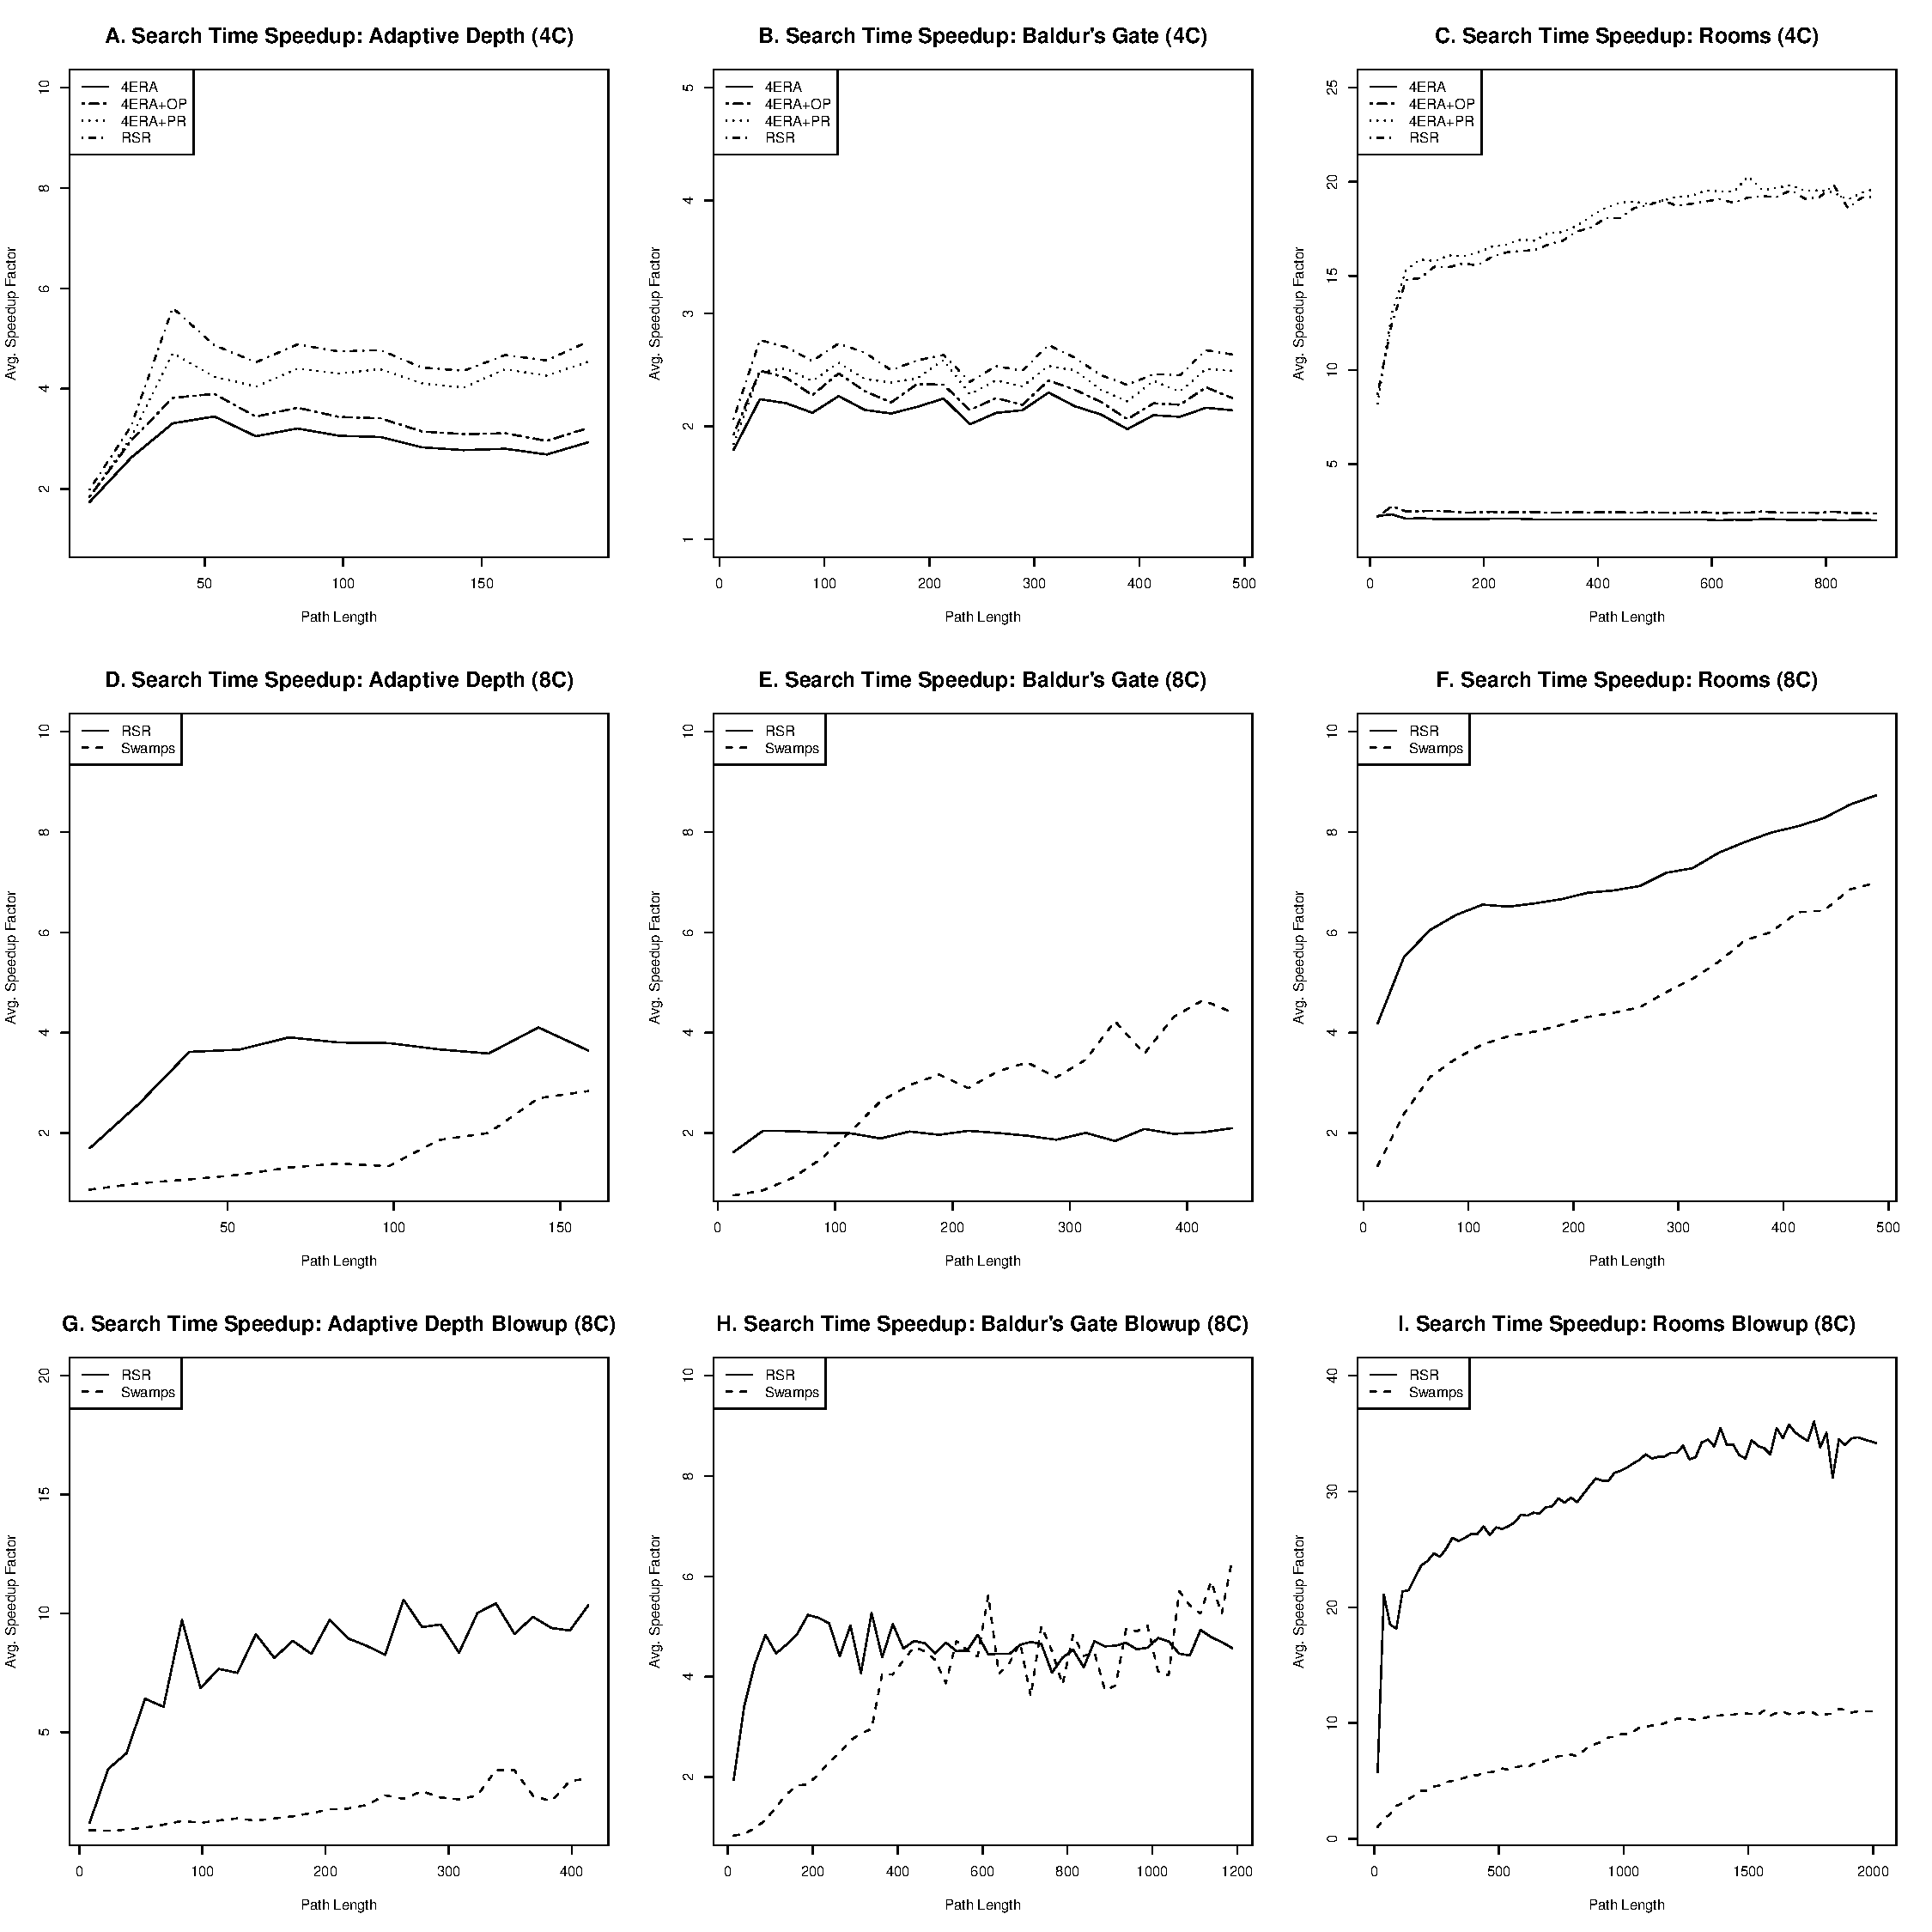
\includegraphics[width=1.90\columnwidth, trim = 10mm 10mm 10mm 0mm]{diagrams/speedup.pdf}
       \end{center}
       \caption{Average A* speedup on each of our three benchmarks. 
		Results are given in terms of search time.}
\label{fig-speedup}
\end{figure*}

\par
\textbf{Comparison with 4ERR and Impact of PR and OP:}
As per Figure \ref{fig-speedup} (A to C), we note is that RSR shows a convincing 
speed-up improvement over 4ERR and all its variants across all input maps.
This allows us to conclude that that RSR is the better choice on 4-connected maps.
\par
When analysing the impact of each enhancement, we note that 4ERR+PR yielded the
biggest improvement on all three benchmarks.
The most dramatic example can be seen on the Rooms benchmark (Figure \ref{fig-speedup}C) 
where 4ERR+PR speeds up A* by over 18 times.
By comparison, 4ERR+OP yields much smaller gains across the same
benchmarks: usually beating 4ERR by between 10-12\%.
%In an additional experiment, we evaluated the impact of OP on 8-connected
%grids and observed that its contribution to speedup was more significant than in 
%the 4-connected case.
%This can be explained as follows: on 4-connected maps, 4ERR maintains a very low
%branching factor, which is comparable (and even slightly better) than the branching
%factor on the original map. 
%On the other hand, 8ERR (i.e. RSR without OP and PR speedup enhancements) 
%can introduce larger branching factors. Therefore, there are more opportunities for 
%online pruning in the latter case. 
%Other details (and charts) are left out because of room limitations.
\par
Finally, it is interesting to note the sometimes large performance variation 
from one benchmark to another. This is indicative of how effectively we can 
decompose the different maps into rectangular shaped regions.
For example, the maps in the Rooms set are highly suited to this approach but those
from Baldur's Gate, which have an unusual 45-degree orientation, are not.
\par
\textbf{Comparison to Swamps:}
Figure \ref{fig-speedup} (D to F) gives search time speedup results for both RSR
and Swamps running on the 8-connected variants of our three benchmark problem
sets.  The results are mixed; on Adaptive Depth and Rooms, RSR achieves higher
speedups and is shown consistently better than Swamps. However, on Baldur's
Gate, this trend is reversed.  
It is interesting to note that on the
benchmarks where RSR performs well there are usually large open areas and the
terrain can often be naturally decomposed into rectangular rooms.  This is not
true for the Baldur's Gate benchmark where Swamps-based pruning appears to be
more effective.
\par
To test this hypothesis we scaled each map in every benchmark by a factor of 3
and generated a new set of 100 problem instances per map. 
Scaling has the effect of producing larger open areas and allows 
us to measure the impact of this variable on search time speedup.
We present our findings in  Figure \ref{fig-speedup} (G to I).
We observe that while the maximum speedup achieved by both algorithms has
increased, the gain for Swamps is very small while RSR shows dramatic
improvement.
Infact, if we limit our attention to problems of similar length to those seen 
on the original maps we notice that the performance of Swamps actually
decreases.
\par
The observed performance characteristics are not unexpected: 
Swamps prune out areas that can be avoided without introducing a detour while 
rectangle-based symmetry reduction allows for a faster exploration of areas that need to be searched.
Since it appears that the two algorithms are orthogonal, a natural extension of this work would 
be to combine the two: 
first, apply 4(or 8)ERR+PR (as appropriate) to a grid in order to eliminate as many interior nodes 
as possible; then, apply a Swamps-based decomposition to the resultant graph.
